

	In order to allow the user to set up complex signal routing configurations, an analog signal routing matrix needed to be designed.  To keep the modules simple and independent while still providing a large variety of routing options, each module is equipped with a 2x2 mixer.  These options become available when the modules are connected together as in Figure \ref{fig:system_block}.

	\subsubsection{Routing Architecture}

	Each module contains a two input, two output mixer. Each of the two outputs 1 and 2 can be connected to either input $A$ or $B$, as well as the sum of the two inputs $A + B$.  Table \ref{tab:routing_outputs} shows the possible outputs.  As can be seen, there are only three signals that must be available for the output.

	\begin{table}
	\begin{center}
	\begin{tabular}{ |c|c c| }
	\hline
	 Permutation & Output 1 & Output 2 \\ 
	 \hline
	 1 	& $A$ 	& $A$ \\  
	 2 	& $A$ 	& $B$ \\
	 3	& $A$ 	& $A+B$ \\
	 4	& $B$ 	& $A$ \\
	 5	& $B$ 	& $B$ \\
	 6	& $B$ 	& $A+B$ \\
	 7	& $A+B$ & $A$ \\
	 8	& $A+B$ & $B$ \\
	 9	& $A+B$ & $A+B$ \\
	 \hline
	\end{tabular}
	\caption{List of the $2^3$ possible output signals for each routing module.}
	\label{tab:routing_outputs}
	\end{center}
	\end{table}

	The routing mechanism was designed with this in mind.  For the same reasons that relays were chosen to actuate the signal switching in the hot swapping receiver subsystem, they are also used here.  This is essential especially when an output is connected directly to an input, such as permutation 2 in Table \ref{tab:routing_outputs}, which will preserve both the SNR and frequency content of the signals in addition to the signal's output impedance.  However, when a summed output is chosen ($A+B$), the signals must necessarily pass through a summing amplifier, which will result in a low impedance output anyways.  In this instance, the use of a mechanical relay is not strictly necessary.

	The specific implementation of the routing subsystem is shown in Figure \ref{fig:routingschem}.  Each output selector is in essence a three-to-one analog multiplexer.  The requirement for mechanical relays when the sum output is not selected requires the use of mechanical relays throughout, as each can only switch between two inputs.  Thus, each three-to-one multiplexer includes two of the same DPDT relays used for the receivers, despite not all of the throws being in use, as they were cheaper than any SPDT relay.  Using the same UD2-5SNU relays also minimizes additional components on the BOM.  The use of latching relays here is even more beneficial than in the receiver, as these relays will likely be set in a position for long periods of time, so the reduced current and heat dissipation compared to a non-latching relay is very beneficial.

	To generate the summed $A+B$ signal, a standard inverted summing amplifier is used.  The resistors were chosen to each be $10K\Omega$ so that each input is at unity gain.  Higher resistor values were avoided to reduce thermal noise.  However, the input impedance to the inverted amplifier is just the value of the input resistor, so non-inverting op-amp buffers are required to prevent preceding circuits on $A$ and $B$ from interacting with the summing amplifier, which in this case is undesirable.  As this already requires three op-amps and the output signal would be inverted, an additional unity gain inverted buffer is used at the output to re-invert the signal, resulting in $A+B$.

	The $A$ and $B$ inputs are each connected through a decoupling capacitor to their respective op-amp buffer inputs, and are pulled to the reference voltage via 1M resistors.  The 1M resistors were chosen to prevent the $A$ and $B$ signals from being heavily loaded down, especially when the signal passes a number of these between the input and output.  When the signal sees several of these in parallel, the equivalent resistance decreases quickly, which can result in issues, so a larger biasing resistance is desirable.  A large resistor value here also means the capacitance of the decoupling capacitor can be less to maintain a similar cutoff frequency, and it will be cheaper to have a higher quality plastic film or C0G ceramic capacitor in a smaller value.  The limit to choosing a very large resistor is the thermal noise, which may become a concern even with this value.  If this becomes an issue, the values can be adjusted once the board has been fabricated.  The cutoff frequency for the high pass filter formed by pull-up resistor and the decoupling capacitor should have its cutoff frequency on the order of 5-10Hz so it will pass the full audio range.  For a 1\Mohm resistor, this means

	$$ C = \frac{1}{2\pi R F_c} = \frac{1}{2\pi (1 \text{\Mohm}) (10 \text{Hz})} = 15.8 \text{nF}$$

	Because this is on the high end of the frequency range, the next larger standard value capacitor, 0.022\uF, is used.  Kemet offers a 0.022\uF film capacitor in through hole mounting for just \$0.25.  The film capacitors are more linear and have lower ESR and self inductance than typical ceramic caps, making them suitable for audio signal path usage.  The resistors can be standard.

	The op-amp selected should have low noise, low input bias current to prevent loading the input signal lines, and a rail-to-rail output to maximize headroom.  For op-amps compatible with a supply of 24V or more, Texas Instrument's OPA1679IDR is a good candidate.  At \$1.20 from Digikey, it is not cheap, but its datasheet claims 0.0001\% THD+N, a 10 pA max input bias current, and voltage output within 800mV of each rail \cite{OPA1679IDRdatasheet}.  These specs compare admirably to the TLV4172IDR and OPA4172IDR, each of which are twice the price.  Because there are not too many components in the audio path and its value as a reliable reference is paramount, it is appropriate to use more expensive and higher quality parts here.  The schematic for the analog signal routing subsystem is shown in Figure \ref{fig:routingschem}.  

	\begin{sidewaysfigure}
		\centering
		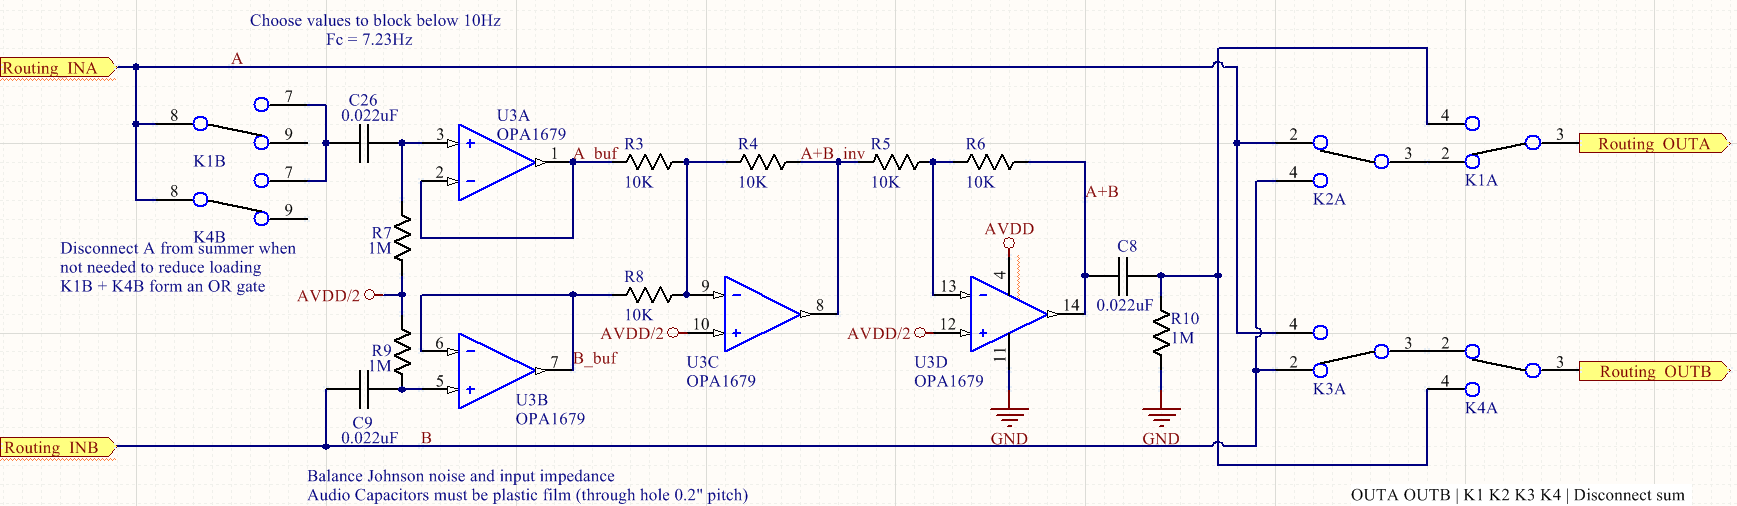
\includegraphics[width = \textwidth]{PR4Images/RoutingSchem.PNG}
		\caption{Schematic of analog signal routing subsystem.  Note that the second halves of two out of the four routing relays are in use.  The relays associated with choosing between a summed output or not are used to create an OR gate which will disconnect the biasing resistors from the $A$ signal, reducing the loading whenever the summer is not needed.}
		\label{fig:routingschem}
	\end{sidewaysfigure}

	\subsubsection{Analog Voltage Supply}

	
	This summing amplifier and related circuitry requires its own analog supply voltage.  In the worst case, the maximum voltage swing of each input signal $A$ and $B$ should be no more than 18Vpp, which is the maximum supply voltage available to a pedal from a receiver.  This means that the summing amplifier should ideally be able to swing 36Vpp.  However, the power supply currently being used provides 24VDC.  This means that without modification, the summing amplifier will not be able to sum all possible signals without clipping.

	There are several possible solutions to this issue.  One would be to change the device's power supply.  Moving to a chassis mount 48V supply like Mean Well's LRS-150-48 \cite{datasheet:LRS-150-48} (\$22.50 from Digikey \cite{digikey}) would allow for plenty of headroom and could provide much more current (in this case 3.3A), enough for six pedals each drawing 500 mA while leaving some budget for the device's own circuits.  A new power supply could be chosen to avoid the issue of switching noise in the audio range; the switching frequency of the LRS-150-48 is 65kHz, well above the audio spectrum.  Linear regulators could be used to drop the input voltage to the desired level, in this case just above 36V.  This supply could then be split with a resistive divider to provide the virtual ground needed for the op amp summer.  Brick-type supplies in this voltage and current range are prohibitively expensive, such as the PSA120U-480L6 from Philhong USA for \$38 \cite{digikey}.

	A second option would be designing an on-board boost-buck converter to create the desired supply voltages.  In this case, this switching supply could be used to generate an arbitrary voltage, so a bipolar 18V or 24V set of rails could be created.  This would allow for sufficient headroom for the summing amplifier, and by virtue of the bipolar supply would not require AC coupling the summed signals to a virtual ground: they could remain DC coupled.  A switching supply would also be more efficient than a linear regulator.  However, the added complexity of implementing a switching voltage regulator, is probably not worth the benefits.  Noise from the on-board supply would need to be carefully controlled so as to avoid corrupting the audio signals.  In addition, a linear regulator would likely still be used to really clean up the residual ripple from a switching regulator.

	The third option is simply using a linear regulator to even out the current 24V supply and allowing the summing amplifier to clip at a lower voltage.  This is not as big an issue as it seems at first.  Though the worst case scenario is two 18Vpp signals being summed in phase, this would require the user to be using two pedals in 18V mode at full output level.  The more likely use case with two 9V pedals would work fine with the 24V supply.  If the user does cause the summing amplifier to clip, they can simply reduce the output level of the two pedals.  In addition, if the amplifier were able to sum two outputs to 36Vpp, this would cause the next pedal in the chain to clip as well because of its voltage could be 18V at maximum, so the 36Vpp output would only be usable at the input of the amplifier where it would not clip the amplifier input.  This is also the simplest option, as it requires only a linear regulator to clean up the 24V input and a resistive divider to generate the virtual ground reference voltage.  

	\begin{table}
	\begin{center}
	\begin{tabular}{|c|p{2in} p{2in}|}
	\hline
	Option & Pros & Cons \\
	\hline
	Change Power Supply 	& Allow increased headroom for summing amplifier.  Increase current capacity for entire system.  Possible to fix switching noise issue. 
								& Potentially expensive for quality supply with the required high current and voltage.  No guarantee that all issues will be solved. \\
	On-board Switcher 		& Bipolar supply possible for DC coupling.  Arbitrary headroom for this application.  More efficient than linear regulators. 	
								& Complicated.  Potential for its own noise issues would require mitigation. \\
	No Action 				& Easy.  Cheap.  Still satisfies most operating conditions. Low Noise.
								& Limited headroom.  Inefficient. \\
	\hline
	\end{tabular}
	\caption{Summary of analog supply voltage regulation options.}
	\label{tab:pwrsupplyproscons}
	\end{center}
	\end{table}

	Because of the simplicity of the third option and its relatively limited negative effects, this method was chosen to provide the supply for the summing amplifier.  To maximize the dynamic range of the summing amplifier, the regulated supply rail should be as close as possible to the 24V input.  The 200mV noise spec on the power supply means that the regulator must drop at least 200mV.  An adjustable regulator would be useful here to precisely set the output voltage.  The LM317 adjustable regulator used for the receiver is one option.  However, it's minimum 3V drop between input and output means that the analog supply rail cannot be set any higher than 21V \cite{LM317datasheet}.  This decreased headroom is not desirable, so a lower dropout device would be preferable.  The LM2931C is an adjustable low dropout voltage regulator which can be set output anywhere from 3 to 24V with a maximum dropout voltage of just 0.6V, about one diode drop.  This means that the analog supply voltage AVDD can be set very close to the 24V input.

	The LM2931C's datasheet provides design guidelines for setting the output voltage, but it follows the same principle as the LM317 divider used for the receiver.  The datasheet gives the following equation to set the output \cite{LM2931datasheet}:

	$$ V_{out} = V_{ref} \left( 1 + \frac{R_2}{R_1} \right) + I_{adj}R_2 $$

	which also accounts for the small current on the ADJ pin.  The datasheet also suggests keeping

	$$ 22.5\text{\kohm} \ge \frac{R_1R2}{R_1 + R_2} $$

	According to the electrical characteristics page, the reference voltage $V_{ref} = 1.2V$, and the adjust pin current $I_{adj} = 0.2\mu$A.  Setting $R_1 = 27$\kohm and $R_2 = 487$\kohm gives an output voltage of 23V, which is ideal.  The 487\kohm resistor is not one of the standard values, but slight adjustments in resistance to get to a nearby value cause too much of a change in voltage.  The output must also have a capacitive load on the order of 10\uF for stability.  Figure \ref{fig:AVDDreg} shows the circuit implementation of the regulator.

	\begin{figure}
		\centering
		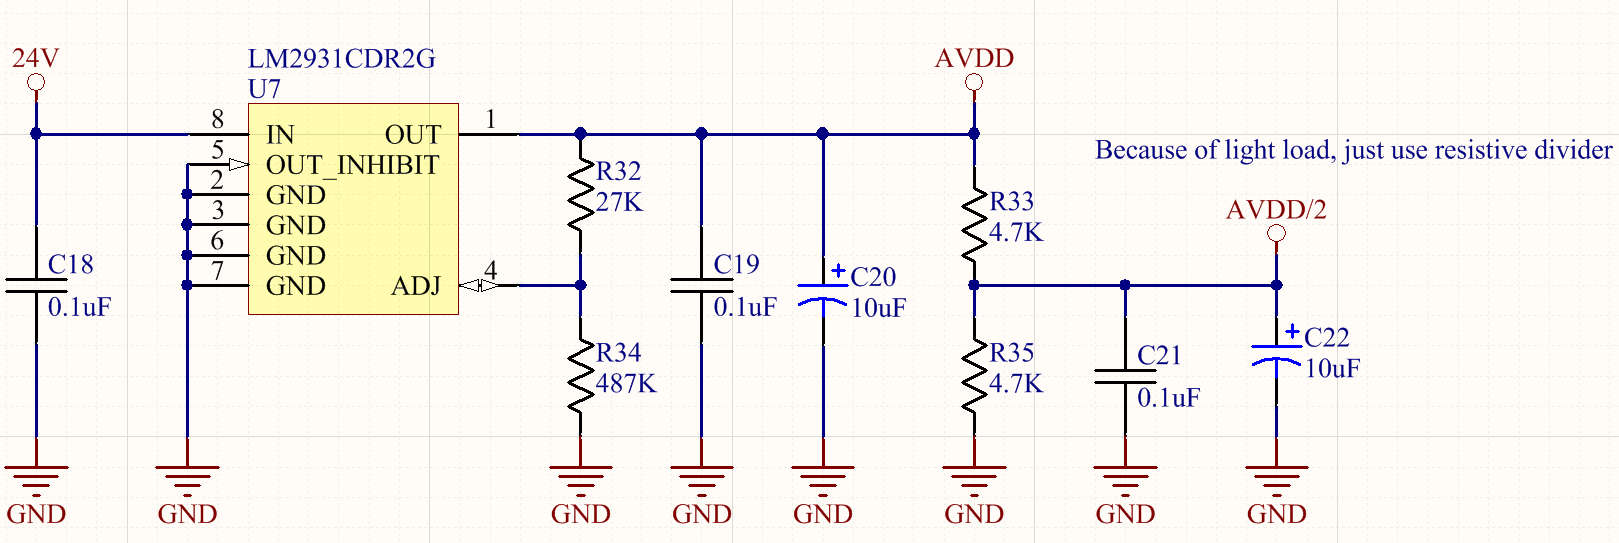
\includegraphics[width = \textwidth]{PR4Images/AVDDregulator.PNG}
		\caption{AVDD regulator design using LM2931C low voltage adjustable regulator and a resistive divider to provide a large split supply.}
		\label{fig:AVDDreg}
	\end{figure}

	From this analog supply voltage, a virtual ground can be produced from a simple resistive divider circuit.  Though in theory this is susceptible to sagging due to large current loads, this should not be an issue for this application because the reference voltage is connected only to the inputs of two op-amps, and tied to the audio signal through large resistors.
